\documentclass{ximera}

%\usepackage{todonotes}

\newcommand{\todo}{}

\usepackage{esint} % for \oiint
\ifxake%%https://math.meta.stackexchange.com/questions/9973/how-do-you-render-a-closed-surface-double-integral
\renewcommand{\oiint}{{\large\bigcirc}\kern-1.56em\iint}
\fi


\graphicspath{
  {./}
  {ximeraTutorial/}
  {basicPhilosophy/}
  {functionsOfSeveralVariables/}
  {normalVectors/}
  {lagrangeMultipliers/}
  {vectorFields/}
  {greensTheorem/}
  {shapeOfThingsToCome/}
  {dotProducts/}
  {partialDerivativesAndTheGradientVector/}
  {../productAndQuotientRules/exercises/}
  {../normalVectors/exercisesParametricPlots/}
  {../continuityOfFunctionsOfSeveralVariables/exercises/}
  {../partialDerivativesAndTheGradientVector/exercises/}
  {../directionalDerivativeAndChainRule/exercises/}
  {../commonCoordinates/exercisesCylindricalCoordinates/}
  {../commonCoordinates/exercisesSphericalCoordinates/}
  {../greensTheorem/exercisesCurlAndLineIntegrals/}
  {../greensTheorem/exercisesDivergenceAndLineIntegrals/}
  {../shapeOfThingsToCome/exercisesDivergenceTheorem/}
  {../greensTheorem/}
  {../shapeOfThingsToCome/}
  {../separableDifferentialEquations/exercises/}
  {vectorFields/}
}

\newcommand{\mooculus}{\textsf{\textbf{MOOC}\textnormal{\textsf{ULUS}}}}

\usepackage{tkz-euclide}
\usepackage{tikz}
\usepackage{tikz-cd}
\usetikzlibrary{arrows}
\tikzset{>=stealth,commutative diagrams/.cd,
  arrow style=tikz,diagrams={>=stealth}} %% cool arrow head
\tikzset{shorten <>/.style={ shorten >=#1, shorten <=#1 } } %% allows shorter vectors

\usetikzlibrary{backgrounds} %% for boxes around graphs
\usetikzlibrary{shapes,positioning}  %% Clouds and stars
\usetikzlibrary{matrix} %% for matrix
\usepgfplotslibrary{polar} %% for polar plots
\usepgfplotslibrary{fillbetween} %% to shade area between curves in TikZ
%\usetkzobj{all}
\usepackage[makeroom]{cancel} %% for strike outs
%\usepackage{mathtools} %% for pretty underbrace % Breaks Ximera
%\usepackage{multicol}
\usepackage{pgffor} %% required for integral for loops



%% http://tex.stackexchange.com/questions/66490/drawing-a-tikz-arc-specifying-the-center
%% Draws beach ball
\tikzset{pics/carc/.style args={#1:#2:#3}{code={\draw[pic actions] (#1:#3) arc(#1:#2:#3);}}}



\usepackage{array}
\setlength{\extrarowheight}{+.1cm}
\newdimen\digitwidth
\settowidth\digitwidth{9}
\def\divrule#1#2{
\noalign{\moveright#1\digitwidth
\vbox{\hrule width#2\digitwidth}}}




% \newcommand{\RR}{\mathbb R}
% \newcommand{\R}{\mathbb R}
% \newcommand{\N}{\mathbb N}
% \newcommand{\Z}{\mathbb Z}

\newcommand{\sagemath}{\textsf{SageMath}}


%\renewcommand{\d}{\,d\!}
%\renewcommand{\d}{\mathop{}\!d}
%\newcommand{\dd}[2][]{\frac{\d #1}{\d #2}}
%\newcommand{\pp}[2][]{\frac{\partial #1}{\partial #2}}
% \renewcommand{\l}{\ell}
%\newcommand{\ddx}{\frac{d}{\d x}}

% \newcommand{\zeroOverZero}{\ensuremath{\boldsymbol{\tfrac{0}{0}}}}
%\newcommand{\inftyOverInfty}{\ensuremath{\boldsymbol{\tfrac{\infty}{\infty}}}}
%\newcommand{\zeroOverInfty}{\ensuremath{\boldsymbol{\tfrac{0}{\infty}}}}
%\newcommand{\zeroTimesInfty}{\ensuremath{\small\boldsymbol{0\cdot \infty}}}
%\newcommand{\inftyMinusInfty}{\ensuremath{\small\boldsymbol{\infty - \infty}}}
%\newcommand{\oneToInfty}{\ensuremath{\boldsymbol{1^\infty}}}
%\newcommand{\zeroToZero}{\ensuremath{\boldsymbol{0^0}}}
%\newcommand{\inftyToZero}{\ensuremath{\boldsymbol{\infty^0}}}



% \newcommand{\numOverZero}{\ensuremath{\boldsymbol{\tfrac{\#}{0}}}}
% \newcommand{\dfn}{\textbf}
% \newcommand{\unit}{\,\mathrm}
% \newcommand{\unit}{\mathop{}\!\mathrm}
% \newcommand{\eval}[1]{\bigg[ #1 \bigg]}
% \newcommand{\seq}[1]{\left( #1 \right)}
% \renewcommand{\epsilon}{\varepsilon}
% \renewcommand{\phi}{\varphi}


% \renewcommand{\iff}{\Leftrightarrow}

% \DeclareMathOperator{\arccot}{arccot}
% \DeclareMathOperator{\arcsec}{arcsec}
% \DeclareMathOperator{\arccsc}{arccsc}
% \DeclareMathOperator{\si}{Si}
% \DeclareMathOperator{\scal}{scal}
% \DeclareMathOperator{\sign}{sign}


%% \newcommand{\tightoverset}[2]{% for arrow vec
%%   \mathop{#2}\limits^{\vbox to -.5ex{\kern-0.75ex\hbox{$#1$}\vss}}}
% \newcommand{\arrowvec}[1]{{\overset{\rightharpoonup}{#1}}}
% \renewcommand{\vec}[1]{\arrowvec{\mathbf{#1}}}
% \renewcommand{\vec}[1]{{\overset{\boldsymbol{\rightharpoonup}}{\mathbf{#1}}}}

% \newcommand{\point}[1]{\left(#1\right)} %this allows \vector{ to be changed to \vector{ with a quick find and replace
% \newcommand{\pt}[1]{\mathbf{#1}} %this allows \vec{ to be changed to \vec{ with a quick find and replace
% \newcommand{\Lim}[2]{\lim_{\point{#1} \to \point{#2}}} %Bart, I changed this to point since I want to use it.  It runs through both of the exercise and exerciseE files in limits section, which is why it was in each document to start with.

% \DeclareMathOperator{\proj}{\mathbf{proj}}
% \newcommand{\veci}{{\boldsymbol{\hat{\imath}}}}
% \newcommand{\vecj}{{\boldsymbol{\hat{\jmath}}}}
% \newcommand{\veck}{{\boldsymbol{\hat{k}}}}
% \newcommand{\vecl}{\vec{\boldsymbol{\l}}}
% \newcommand{\uvec}[1]{\mathbf{\hat{#1}}}
% \newcommand{\utan}{\mathbf{\hat{t}}}
% \newcommand{\unormal}{\mathbf{\hat{n}}}
% \newcommand{\ubinormal}{\mathbf{\hat{b}}}

% \newcommand{\dotp}{\bullet}
% \newcommand{\cross}{\boldsymbol\times}
% \newcommand{\grad}{\boldsymbol\nabla}
% \newcommand{\divergence}{\grad\dotp}
% \newcommand{\curl}{\grad\cross}
%\DeclareMathOperator{\divergence}{divergence}
%\DeclareMathOperator{\curl}[1]{\grad\cross #1}
% \newcommand{\lto}{\mathop{\longrightarrow\,}\limits}

% \renewcommand{\bar}{\overline}

\colorlet{textColor}{black}
\colorlet{background}{white}
\colorlet{penColor}{blue!50!black} % Color of a curve in a plot
\colorlet{penColor2}{red!50!black}% Color of a curve in a plot
\colorlet{penColor3}{red!50!blue} % Color of a curve in a plot
\colorlet{penColor4}{green!50!black} % Color of a curve in a plot
\colorlet{penColor5}{orange!80!black} % Color of a curve in a plot
\colorlet{penColor6}{yellow!70!black} % Color of a curve in a plot
\colorlet{fill1}{penColor!20} % Color of fill in a plot
\colorlet{fill2}{penColor2!20} % Color of fill in a plot
\colorlet{fillp}{fill1} % Color of positive area
\colorlet{filln}{penColor2!20} % Color of negative area
\colorlet{fill3}{penColor3!20} % Fill
\colorlet{fill4}{penColor4!20} % Fill
\colorlet{fill5}{penColor5!20} % Fill
\colorlet{gridColor}{gray!50} % Color of grid in a plot

\newcommand{\surfaceColor}{violet}
\newcommand{\surfaceColorTwo}{redyellow}
\newcommand{\sliceColor}{greenyellow}




\pgfmathdeclarefunction{gauss}{2}{% gives gaussian
  \pgfmathparse{1/(#2*sqrt(2*pi))*exp(-((x-#1)^2)/(2*#2^2))}%
}


%%%%%%%%%%%%%
%% Vectors
%%%%%%%%%%%%%

%% Simple horiz vectors
\renewcommand{\vector}[1]{\left\langle #1\right\rangle}


%% %% Complex Horiz Vectors with angle brackets
%% \makeatletter
%% \renewcommand{\vector}[2][ , ]{\left\langle%
%%   \def\nextitem{\def\nextitem{#1}}%
%%   \@for \el:=#2\do{\nextitem\el}\right\rangle%
%% }
%% \makeatother

%% %% Vertical Vectors
%% \def\vector#1{\begin{bmatrix}\vecListA#1,,\end{bmatrix}}
%% \def\vecListA#1,{\if,#1,\else #1\cr \expandafter \vecListA \fi}

%%%%%%%%%%%%%
%% End of vectors
%%%%%%%%%%%%%

%\newcommand{\fullwidth}{}
%\newcommand{\normalwidth}{}



%% makes a snazzy t-chart for evaluating functions
%\newenvironment{tchart}{\rowcolors{2}{}{background!90!textColor}\array}{\endarray}

%%This is to help with formatting on future title pages.
\newenvironment{sectionOutcomes}{}{}



%% Flowchart stuff
%\tikzstyle{startstop} = [rectangle, rounded corners, minimum width=3cm, minimum height=1cm,text centered, draw=black]
%\tikzstyle{question} = [rectangle, minimum width=3cm, minimum height=1cm, text centered, draw=black]
%\tikzstyle{decision} = [trapezium, trapezium left angle=70, trapezium right angle=110, minimum width=3cm, minimum height=1cm, text centered, draw=black]
%\tikzstyle{question} = [rectangle, rounded corners, minimum width=3cm, minimum height=1cm,text centered, draw=black]
%\tikzstyle{process} = [rectangle, minimum width=3cm, minimum height=1cm, text centered, draw=black]
%\tikzstyle{decision} = [trapezium, trapezium left angle=70, trapezium right angle=110, minimum width=3cm, minimum height=1cm, text centered, draw=black]


\title{Categories}

\begin{document}

\begin{abstract}
elementary library
\end{abstract}
\maketitle




Success at analyzing functions rests entirely on our ability to recognize what type of function we have.  Categorizing functions is the quickest and best way of gaining information about our function.

Our library of elementary functions gives us a wonerful filter to begin idenitfying functions.  \\



\begin{template}  \textbf{\textcolor{blue!55!black}{Constant Functions}} \\



Constant funtions are functions which give the same value for all domain numbers. \\


They can be represented by formulas that look like


\[ f(x) = C  \,  \text{ for all } x  \, \text{ in the domain. }   \]



\end{template}



The natural domain of a constant function is all real numbers.  However, we can always state a restricted domain.




\begin{warning}   \textbf{\textcolor{red!80!black}{can}}  \\

All of our definitions for the elementary functions use the word \textbf{\textcolor{red!80!black}{can}}.


\begin{example}

The function representated by 

\[ f(x) = \frac{x^2 - 1}{x + 1} - x  \,  \text{ on } \,   [0, \infty)   \]

is a constant function.   $-1$ is the only function value.


\end{example}





\begin{example}

The function representated by 

\[ C(\theta) = (\cos(\theta))^2 + (\sin(\theta))^2   \,  \text{ on } \,   (-\infty, \infty)   \]

is a constant function.   $1$ is the only function value.


\end{example}




Constant functions are disguised with many formulas.  They \textbf{\textcolor{red!80!black}{can}} be written in the form $f(x) = C$.



\end{warning}




Graphs of constant functions are horizontal lines.
\[ f(x) = 3\]





\begin{image}
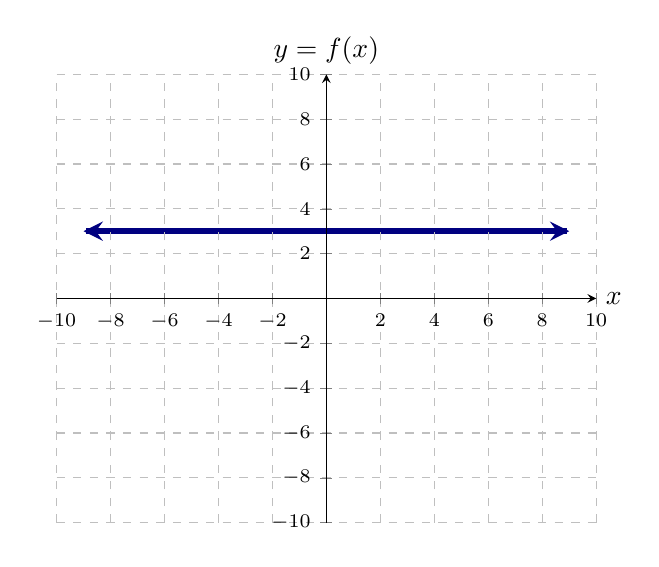
\begin{tikzpicture}
  \begin{axis}[
            domain=-10:10, ymax=10, xmax=10, ymin=-10, xmin=-10,
            axis lines =center, xlabel=$x$, ylabel={$y=f(x)$}, grid = major, grid style={dashed},
            ytick={-10,-8,-6,-4,-2,2,4,6,8,10},
            xtick={-10,-8,-6,-4,-2,2,4,6,8,10},
            yticklabels={$-10$,$-8$,$-6$,$-4$,$-2$,$2$,$4$,$6$,$8$,$10$}, 
            xticklabels={$-10$,$-8$,$-6$,$-4$,$-2$,$2$,$4$,$6$,$8$,$10$},
            ticklabel style={font=\scriptsize},
            every axis y label/.style={at=(current axis.above origin),anchor=south},
            every axis x label/.style={at=(current axis.right of origin),anchor=west},
            axis on top
          ]
          
            
      \addplot [line width=2, penColor, smooth,samples=200,domain=(-9:9),<->] {3};




  \end{axis}
\end{tikzpicture}
\end{image}

















\begin{template}  \textbf{\textcolor{blue!55!black}{Linear Functions}} \\



Linear funtions are functions which exhibit a constant rate of change. \\


They can be represented by formulas that look like


\[ f(x) = m x + b  \,  \text{ for all } x  \, \text{ in the domain. }   \]



\end{template}



The natural domain of a linear function is all real numbers.  However, we can always state a restricted domain.







Graphs of linear functions are lines. 
(This make constant functions special linear functions)
\[ f(x) = 2x - 6\]





\begin{image}
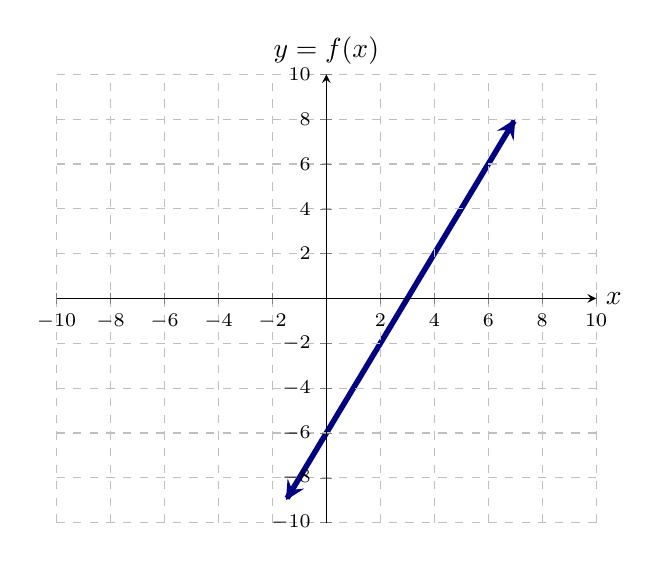
\begin{tikzpicture}
  \begin{axis}[
            domain=-10:10, ymax=10, xmax=10, ymin=-10, xmin=-10,
            axis lines =center, xlabel=$x$, ylabel={$y=f(x)$}, grid = major, grid style={dashed},
            ytick={-10,-8,-6,-4,-2,2,4,6,8,10},
            xtick={-10,-8,-6,-4,-2,2,4,6,8,10},
            yticklabels={$-10$,$-8$,$-6$,$-4$,$-2$,$2$,$4$,$6$,$8$,$10$}, 
            xticklabels={$-10$,$-8$,$-6$,$-4$,$-2$,$2$,$4$,$6$,$8$,$10$},
            ticklabel style={font=\scriptsize},
            every axis y label/.style={at=(current axis.above origin),anchor=south},
            every axis x label/.style={at=(current axis.right of origin),anchor=west},
            axis on top
          ]
          
            
      \addplot [line width=2, penColor, smooth,samples=200,domain=(-1.5:7),<->] {2*x-6};




  \end{axis}
\end{tikzpicture}
\end{image}






Although the definition quotes the slope-intercept form ($m x + b$), this is really not very useful.  In most situations, we do not have the intercept.  Instead, it is more common to have a slope and a random point or just two random points.



\begin{itemize}

\item \textbf{\textcolor{blue!55!black}{Point-Slope:}}  : $(y - y_0) = m (x - x_0)$

\item \textbf{\textcolor{blue!55!black}{Two Points:}}  : $(y - y_0) = \frac{y_1 - y_0}{x_1 - x_0} \, (x - x_0)$

\end{itemize}


All three of these forms are equivalent.  They can all be rearranged into the form of the others.  They are all reflecting the geometry of lines.  


On the other hand, we have seen that the analysis of functions often begins with zeros.  Products of factors is a preferred form.  With that in mind, linear functions can be written in factored form.


\[  f(x) = a (x - z_0)  \]

Where $a$ is the leading coefficient and $z_0$ is the zero of the function.





\begin{itemize}

\item $a = m$, the rate of change of the function is the slope of the line.

\item $z_0$ is the zero of the linear function, which is visually encoded as the intercept $(z_0, 0)$.

\end{itemize}



\textbf{Note:} Constant functions are linear functions, because they can be written as $L(x) = 0 x + C$. \\












\begin{template}  \textbf{\textcolor{blue!55!black}{Quadratic Functions}} \\



Quadratic funtions are the next level of polynomial. \\


They can be represented by formulas that look like


\[ f(x) = a \, x^2 + b \, x + c  \,  \text{ for all } x  \, \text{ in the domain. }   \]



\end{template}



The natural domain of a quadratic function is all real numbers.  However, we can always state a restricted domain.







Graphs of quadratic functions are parabolas. 
\[ f(x) = x^2 + x - 6\]





\begin{image}
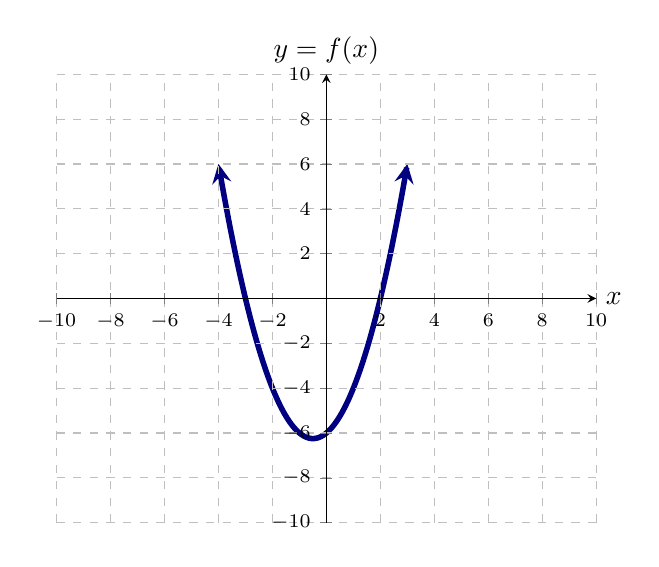
\begin{tikzpicture}
  \begin{axis}[
            domain=-10:10, ymax=10, xmax=10, ymin=-10, xmin=-10,
            axis lines =center, xlabel=$x$, ylabel={$y=f(x)$}, grid = major, grid style={dashed},
            ytick={-10,-8,-6,-4,-2,2,4,6,8,10},
            xtick={-10,-8,-6,-4,-2,2,4,6,8,10},
            yticklabels={$-10$,$-8$,$-6$,$-4$,$-2$,$2$,$4$,$6$,$8$,$10$}, 
            xticklabels={$-10$,$-8$,$-6$,$-4$,$-2$,$2$,$4$,$6$,$8$,$10$},
            ticklabel style={font=\scriptsize},
            every axis y label/.style={at=(current axis.above origin),anchor=south},
            every axis x label/.style={at=(current axis.right of origin),anchor=west},
            axis on top
          ]
          
            
      \addplot [line width=2, penColor, smooth,samples=200,domain=(-4:3),<->] {x^2 + x -6};




  \end{axis}
\end{tikzpicture}
\end{image}






Although the definition quotes the standard form ($a x^2 + b x + c$), there are more useful forms. 





\begin{itemize}

\item \textbf{\textcolor{blue!55!black}{Vertex Form:}}  $a (x - h)^2 + k$ 

\item \textbf{\textcolor{blue!55!black}{Factored Form:}}  $a (x - r_1)(x - r_2)$ 

\end{itemize}








\subsection{Polynomial Functions}


\begin{template}  \textbf{\textcolor{blue!55!black}{Polynomial Functions}} \\



Constant, Linear, and Quadratic funtions are examples of polynomials. \\


Polynomials can be represented by formulas that look like


\[ f(x) = a_n x^n + a_{n-1} x^{n-1} + \cdots + a_1 x + a_0  \,  \text{ for all } x  \, \text{ in the domain. }   \]



\end{template}




The natural domain of a polynomial functions is all real numbers.  However, we can always state a restricted domain.




Although the definition quotes the standard form for a polynomial, the factored form is better suited for our analysis.

\[
p(x) = a (x - r_1)^{e_1} (x - r_2)^{e_2} \cdots (x - r_{k-1})^{e_{k-1}} (x - r_k)^{e_k}  
\]


\begin{itemize}
\item $r_1, r_2, \cdots r_k$ are the unique roots (zeros) of the polynomial.
\item $e_1, e_2, \cdots e_k$ are the exponents of the factors. They are called \textit{multiplicities}.
\end{itemize}



\begin{example}

If is difficult to tell anything from the standard form of this polynomial.

\[
x^8 - 22 x^7 +145 x^6 - 6 x^5 - 2997 x^4 + 6774 x^3 + 7931 x^2 - 15386 x - 13720
\]



Our analysis will benefit greatly from the factored form.


\[
(x+4) (x+1)^2 (x-2) (x-5) (x-7)^3
\]




\end{example}




















\subsection{Rational Functions}




\begin{template}  \textbf{\textcolor{blue!55!black}{Rational Functions}} \\



Rational functions are quotients of polynomials. \\


Rational functions can be represented by formulas that look like


\[ 
f(x) = \frac{ a_n x^n + a_{n-1} x^{n-1} + \cdots + a_1 x + a_0 } {b_m x^m + b_{m-1} x^{m-1} + \cdots + b_1 x + b_0}
\]


\[  \text{ for all } x  \, \text{ in the domain. }   \]



\end{template}




The natural domain of a polynomial functions is all real numbers except the roots (zeros) of the polynomial in the denominator.  However, we can always state a restricted domain.








Although the definition quotes the standard form for a polynomial, the factored form is better suited for our analysis.

\[
p(x) = \frac{ a (x - r_1)^{e_1} (x - r_2)^{e_2} \cdots  (x - r_k)^{e_k} } { b (x - s_1)^{f_1} (x - s_2)^{f_2} \cdots  (x - s_h)^{f_h} }
\]








\begin{itemize}
\item The zeros (roots) of the polynomial in the numerator are the zeros of the rational function.
\item The zeros (roots) of the polynomial in the denominator are the singularities of the rational function.
\end{itemize}





















\subsection{Exponential Functions}










\begin{template}  \textbf{\textcolor{blue!55!black}{Exponential Functions}} \\


Exponential functions are characterized by a constant \textit{percentage} growth rate. \\


We have several thoughts about exponential functions.

First, we have the basic expnential function, which has a formula like, $f(x) = b^x$ with $b > 0$. 
This give us a basic feeling for the behavior of exponential functions.



for example $f(x) = e^x$:


\begin{image}
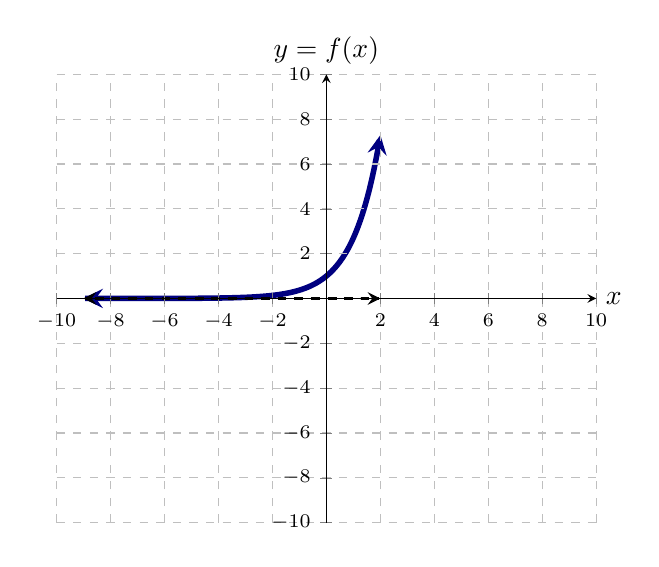
\begin{tikzpicture}
  \begin{axis}[
            domain=-10:10, ymax=10, xmax=10, ymin=-10, xmin=-10,
            axis lines =center, xlabel=$x$, ylabel={$y=f(x)$}, grid = major, grid style={dashed},
            ytick={-10,-8,-6,-4,-2,2,4,6,8,10},
            xtick={-10,-8,-6,-4,-2,2,4,6,8,10},
            yticklabels={$-10$,$-8$,$-6$,$-4$,$-2$,$2$,$4$,$6$,$8$,$10$}, 
            xticklabels={$-10$,$-8$,$-6$,$-4$,$-2$,$2$,$4$,$6$,$8$,$10$},
            ticklabel style={font=\scriptsize},
            every axis y label/.style={at=(current axis.above origin),anchor=south},
            every axis x label/.style={at=(current axis.right of origin),anchor=west},
            axis on top
          ]
          
            
      \addplot [line width=2, penColor, smooth,samples=200,domain=(-9:2),<->] {2.7^x};
      \addplot [line width=1, black, dashed,samples=200,domain=(-9:2),<->] {0};




  \end{axis}
\end{tikzpicture}
\end{image}















Secondly, we have four basic forms of the basic exponential funciton that illustrate the basic variations of the basic behavior.

\begin{itemize}
\item $f(x) = e^x$ 
\item $f(x) = e^{-x}$ 
\item $f(x) = -e^x$ 
\item $f(x) = -e^{-x}$ 
\end{itemize}






Finally, we include shifting and stretching, which algebraically is described by compositions with linear functions.


\[ f(x) = a \, e^{b \, x + c} + d = L_o \circ E \circ L_i\]

\[
\text{ where } \,  E(y) = e^y   \,  \text{ and } \,   L_o(t) = a \, t + d    \,  \text{ and } \,   L_i(v) = b \, v + c
\]



Strictly speaking, vertical shifts are not allowed for exponential functions.  We call them \textit{shifted exponential functions}.  However, nobody is going to complain if we just called them exponential functions.






\end{template}





The natural domain of an exponential function is all real numbers.  However, we can always state a restricted domain. \\









\subsection{Logarithmic Functions}








\begin{template}  \textbf{\textcolor{blue!55!black}{Logarithmic Functions}} \\


Logarithmic function are the inverse functions of exponential functions. \\


We have several thoughts about logarithmic functions.

First, we have the basic logarithmic function, which has a formula like, $f(x) = \log_b(x)$ with $b > 0$. 
This give us a basic feeling for the behavior of exponential functions.



for example $f(x) = \ln(x)$:


\begin{image}
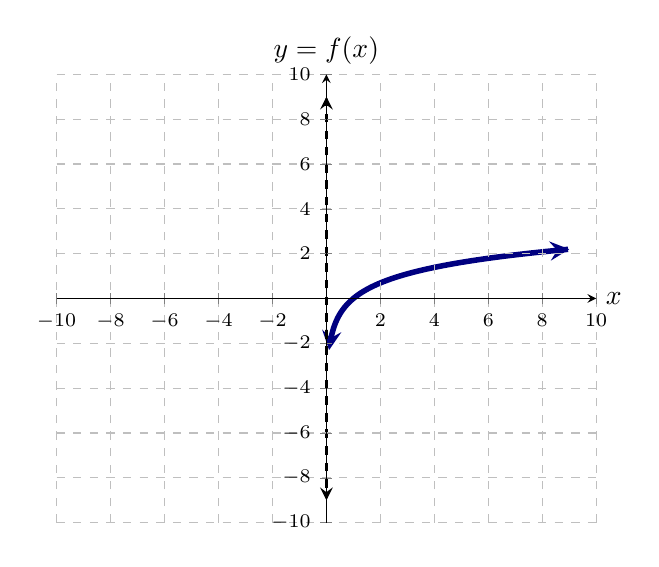
\begin{tikzpicture}
  \begin{axis}[
            domain=-10:10, ymax=10, xmax=10, ymin=-10, xmin=-10,
            axis lines =center, xlabel=$x$, ylabel={$y=f(x)$}, grid = major, grid style={dashed},
            ytick={-10,-8,-6,-4,-2,2,4,6,8,10},
            xtick={-10,-8,-6,-4,-2,2,4,6,8,10},
            yticklabels={$-10$,$-8$,$-6$,$-4$,$-2$,$2$,$4$,$6$,$8$,$10$}, 
            xticklabels={$-10$,$-8$,$-6$,$-4$,$-2$,$2$,$4$,$6$,$8$,$10$},
            ticklabel style={font=\scriptsize},
            every axis y label/.style={at=(current axis.above origin),anchor=south},
            every axis x label/.style={at=(current axis.right of origin),anchor=west},
            axis on top
          ]
          
            
      \addplot [line width=2, penColor, smooth,samples=200,domain=(0.1:9),<->] {ln(x)};
      \addplot [line width=1, black, dashed,samples=200,domain=(-9:9),<->] ({0}, {x});




  \end{axis}
\end{tikzpicture}
\end{image}















Secondly, we have four basic forms of the basic logarithmic funciton that illustrate the basic variations of the basic behavior.

\begin{itemize}
\item $f(x) = \ln(x)$ 
\item $f(x) = \ln(-x)$ 
\item $f(x) = -\ln(x)$ 
\item $f(x) = -\ln(-x)$ 
\end{itemize}






Finally, we include shifting and stretching, which algebraically is described by compositions with linear functions.


\[ f(x) = a \, \ln(b \, x + c) + d = L_o \circ L \circ L_i\]

\[
\text{ where } \,   L(y) = \ln(y)   \,  \text{ and } \,    L_o(t) = a \, t + d    \,  \text{ and } \,   L_i(v) = b \, v + c
\]








\end{template}





















\subsection{Absolute Value Functions}








\begin{template}  \textbf{\textcolor{blue!55!black}{Absolute Functions}} \\



Absolute value functions are usually identified by their vertical bars.





\[ f(x) = a | b x + c | + d = L_o \circ A \circ L_i\]

\[
\text{ where } \,  A(y) = | y |  \,  \text{ and } \,    L_o(t) = a t + d    \,  \text{ and } \,   L_i(v) = b v + c
\]







\end{template}






Unfortunately, our algebra doesn't work vrey well with the vertical bars.  Usually, our first algebraic thought is to get rid of the bars.  This is because the absolute value function is really a piecewise defined function.   \\



\textbf{Notice} that all of our forms are defined by composition with linear functions.  \\

When the ``inside'' or ``outside'' is not a linear function, then we do not have these basic elementary functions. (This is usually the case.)


























\begin{center}
\textbf{\textcolor{green!50!black}{ooooo=-=-=-=-=-=-=-=-=-=-=-=-=ooOoo=-=-=-=-=-=-=-=-=-=-=-=-=ooooo}} \\

more examples can be found by following this link\\ \link[More Examples of Function Forms]{https://ximera.osu.edu/csccmathematics/precalculus2/precalculus2/functionForm/examples/exampleList}

\end{center}







\end{document}
